\chapter{State of the Art}

Graph-based modeling has become a prominent approach for capturing inter-entity dependencies in time-series forecasting, particularly in domains where many variables evolve jointly (e.g., traffic, energy, finance, and recommendation systems) \cite{jin2024survey,li2018dcrnn,yu2018stgcn}. In such settings, the relational structure provides an inductive bias beyond temporal dynamics: a graph specifies which entities are related, whereas temporal models capture how these relationships manifest over time. However, the literature spans substantially different choices regarding how relational structures are obtained (constructed vs.\ learned), what form of representation is extracted (adjacency, node embeddings, or message-passing features), and how tightly this structure is coupled to the forecasting objective \cite{jin2024survey,wu2019graphwavenetdeepspatialtemporal,wu2020connectingdotsmultivariatetime}. These choices directly determine whether the resulting representations are reusable across models and tasks, scalable to large numbers of entities, and robust to non-stationary relations, properties that are central to this study.

Throughout this chapter, the term \emph{graph} primarily denotes a \emph{predictive dependency or similarity structure} used to support forecasting; causal graphs are reviewed separately and treated as requiring stronger assumptions. Moreover, unlike physical networks (e.g., road maps), retail dependencies are typically latent, time-varying, and confounded by exogenous drivers such as promotions and seasonality, often within hierarchical taxonomies (e.g., SKU--category--department) and multi-entity settings (e.g., SKU $\times$ store).

\subsection*{Architectural Paradigms in Graph-Based Forecasting}

To organize prior work, we adopt an architectural lens that separates \emph{how the graph is produced} from \emph{how it is used}. We distinguish two principal paths according to whether the relational structure is constructed independently of the forecasting loss or learned end-to-end as part of the forecaster \cite{jin2024survey}.

\begin{itemize}
    \item \textbf{Path-A (Graph-First Representation Learning Pipelines):}
    Relational dependencies are encoded through an explicitly constructed graph obtained via loss-independent procedures (e.g., correlation filtering, shrinkage estimators, partial correlation networks, or other deterministic/statistical rules) \cite{friedman2008glasso,ledoit2004wellconditioned,tumminello2005pmfg,massara2016tmfg}. The graph functions as a relational prior: it may be used directly as an adjacency or as an input to a graph encoder that produces \emph{node embeddings} (or embedding-like node features) for consumption by a temporal model. Path-A permits the rolling recomputation of graphs and time-varying embeddings; however, the forecasting loss cannot update the graph construction mechanism. This paradigm emphasizes modularity, interpretability, and the reuse of representations. The key property is modularity: the same graph constructor and embedding generator can be reused across forecasting models, horizons, and tasks and can be refreshed over time without backpropagating through the construction rule.
    

    \item \textbf{Path-B (End-to-End Integrated GNN Forecasters):}
    Graph inference, representation learning, and temporal prediction are jointly optimized to minimize forecasting errors \cite{wu2019graphwavenetdeepspatialtemporal,wu2020connectingdotsmultivariatetime,bai2020adaptivegraphconvolutionalrecurrent}. This often yields strong predictive performance; however, the resulting relational structure and representations are typically task-specific and sensitive to training conditions, limiting their reuse and interpretability. Additionally, learning dense inter-variable structures can impose scalability constraints in large entity settings.
\end{itemize}

In line with the research questions, this dissertation focuses on \textbf{Path-A} methods and evaluates them along four criteria: \emph{reusability} of node embeddings across models/tasks and time, \emph{integration strategy} with temporal forecasters (frozen vs.\ rolling/time-varying embeddings), \emph{scalability} with respect to the number of entities and time windows, and \emph{robustness} under nonstationarity, catalog changes, and exogenous drivers such as promotions. Representation quality is operationalized through downstream transferability across forecasters, stability/smoothness over rolling windows, and the consistency/sparsity of induced neighborhoods.

\vspace{0.5em}
\noindent\fbox{%
\begin{minipage}{0.97\linewidth}
\textbf{Evaluation criteria for Path-A pipelines.}
\begin{itemize}
    \item \textbf{Reusability:} transferability across forecasters/tasks; comparability across time windows.
    \item \textbf{Integration:} frozen vs.\ rolling embeddings; injection mechanism into the temporal model.
    \item \textbf{Scalability:} dependence on $|V|$, window length, and graph/embedding recomputation cost.
    \item \textbf{Robustness:} catalog churn, nonstationarity/regime shifts, and confounding by promotions/seasonality.
\end{itemize}
\end{minipage}}
\vspace{0.8em}

\section{Demand-Pattern Categorization via ADI--$CV^2$ Decision Regions}
\label{sec:demand-pattern-categorization-syntetos2005}

Demand-pattern categorization is routinely used in inventory software and spare-parts management to \emph{select an appropriate forecasting and stock-control procedure} for each SKU. However, early schemes (e.g., Williams; Eaves) rely on multi-criterion rules whose cutoff values are typically chosen \emph{heuristically} to fit a particular dataset or managerial intuition, limiting transferability and making the resulting categories method-dependent only in an informal sense.
%
Syntetos et al.\ \cite{syntetos_categorization_2005} formalize an alternative, \textbf{method-driven} view: if categorization is ultimately used for method selection, then categories should be \emph{defined as regions of expected superior forecasting performance}, obtained by comparing competing estimators under an analytically tractable accuracy criterion.
\subsection{ADI--CV\texorpdfstring{\(^2\)}{2} Demand-Pattern Classification}
\label{subsec:adi_cv2_classification_ch2}

A widely adopted classification framework for intermittent demand is based on two summary measures: the Average Demand Interval (ADI) and the squared coefficient of variation of non-zero demand sizes, \(CV^2\). The ADI captures the degree of intermittence by measuring the average interval between non-zero demand occurrences, while \(CV^2\) captures the variability of positive demand sizes.

For an item \(i\), the ADI can be expressed as:

\begin{equation}
    ADI_i = \frac{T_i}{N_i^{+}},
    \label{eq:adi_ch2}
\end{equation}

where \(T_i\) is the total number of observed periods and \(N_i^{+}\) is the number of periods with strictly positive demand. The coefficient of variation is computed using only non-zero demand observations:

\begin{equation}
    CV_i = \frac{\sigma_i^{+}}{\mu_i^{+}},
    \label{eq:cv_ch2}
\end{equation}

where \(\sigma_i^{+}\) and \(\mu_i^{+}\) denote, respectively, the standard deviation and mean of the non-zero demand values. The classification is then based on \(CV_i^2\), rather than on \(CV_i\) directly.

Instead of defining demand categories purely through descriptive or heuristic rules, they derive decision regions by comparing the theoretical mean squared error of different forecasting estimators, including exponentially weighted moving average methods, Croston's method, and the Syntetos--Boylan Approximation. Their analysis shows that stable cutoff values can be obtained around:

\begin{equation}
    ADI^* \approx 1.32,
    \qquad
    (CV^2)^* \approx 0.49.
    \label{eq:adi_cv2_cutoffs_ch2}
\end{equation}
\paragraph{Two-parameter characterization: intermittence and size variability.}
The proposed scheme positions each demand series in the plane spanned by (i) the \textbf{average inter-demand interval} $p$ (a measure of intermittence, i.e., how frequently non-zero demand occurs) and (ii) the \textbf{squared coefficient of variation} $CV^2$ of \emph{non-zero} demand sizes (a measure of transaction-size irregularity).
Larger $p$ indicates sparser arrivals, whereas larger $CV^2$ indicates more volatile non-zero sizes; together they provide a minimal yet operationally meaningful summary of intermittent-demand structure.

\paragraph{Decision regions from theoretical MSE comparisons.}
Syntetos et al.\ derive lead-time MSE expressions for three estimators: (i) EWMA (as a generic baseline), (ii) Croston's method (designed for intermittence), and (iii) the Syntetos--Boylan modification (SBA), proposed as an approximately unbiased alternative to Croston-type forecasting.
Pairwise comparisons of these MSE expressions yield inequalities that delineate regions where one method is theoretically expected to outperform another.
By analysing these inequalities over smoothing constants regarded as realistic for intermittent demand ($\alpha \in [0.05,0.20]$), the authors obtain \emph{stable} cutoff values around
\[
p^\star \approx 1.32,\qquad (CV^2)^\star \approx 0.49,
\]
with only minor shifts across $\alpha$ (reported explicitly in their cutoff table).

A central resulting rule is that, for smoothing constants commonly used in practice, the SBA estimator is expected to dominate for \emph{more intermittent and/or more irregular} series, specifically whenever $p>p^\star$ and/or $CV^2>(CV^2)^\star$. Conversely, in the joint low-intermittence/low-variability corner ($p\le p^\star$ and $CV^2\le (CV^2)^\star$), neither Croston nor SBA can be shown to dominate uniformly; the authors assign this area of indecision to Croston based on numerical analysis, noting that differences are typically small.

\paragraph{Four demand-pattern regions (ADI--$CV^2$ quadrants).}
Combining the two cutoffs partitions the $(p, CV^2)$ space into four regions (Figure~3 in \cite{syntetos2005}), which 
can be noted in the following table:
\begin{table}[h]
\centering
\caption{ADI--$CV^2$ demand-pattern regions.}
\label{tab:adi-cv2-regions}
\begin{tabular}{lllll}
\toprule
\textbf{Area} & \textbf{Label} & \textbf{$p$ (ADI)} & \textbf{$CV^2$} & \textbf{Interpretation} \\
\midrule
1 & Smooth & $p \le 1.32$ & $CV^2 \le 0.49$ & Frequent demand; low non-zero size variability \\
2 & Erratic (not very intermittent) & $p \le 1.32$ & $CV^2 > 0.49$ & Frequent demand; high non-zero size variability \\
3 & Intermittent (not very erratic) & $p > 1.32$ & $CV^2 \le 0.49$ & Infrequent demand; relatively stable non-zero sizes \\
4 & Lumpy & $p > 1.32$ & $CV^2 > 0.49$ & Infrequent demand; highly variable non-zero sizes \\
\bottomrule
\end{tabular}
\end{table}

Importantly, these labels are not introduced as purely descriptive quadrants; they are \emph{induced by relative estimator performance} under the paper's theoretical MSE analysis.

\begin{comment}
\paragraph{Empirical validation on real intermittent-demand series.}
To test whether the theoretical decision rules are reflected in practice, the authors evaluate them on a dataset of 3000 real intermittent-demand series of length 24 months each, considering lead times $L \in \{1,3,5\}$ and smoothing constants $\alpha \in \{0.05,0.10,0.15,0.20\}$.
Using chi-square (and related proportion) tests, they show that empirical MSE outcomes are \emph{not independent} of what the decision regions predict, providing evidence that the proposed cutoffs and region structure constitute a practically meaningful basis for demand-pattern categorization.
\end{comment}

\subsection{Two-Fold Forecasting for Irregular Demand: Occurrence \texorpdfstring{$\rightarrow$}{->} Size}
\label{sec:two-fold-approach-rozanec}

\cite{reframingdemandforecastingtwofold} frame intermittent and lumpy demand as a \emph{compound} forecasting problem driven by a distinct event-generation mechanism that produces many zeros. Building on the Croston-style separation of ``whether'' vs.\ ``how much'', they propose a two-fold decomposition in which (i) \textbf{demand occurrence} is modeled as a \emph{classification} task and (ii) \textbf{non-zero demand size} is modeled as a \emph{regression} task, with forecasts obtained by combining (gating) the size estimate by the predicted occurrence.

The paper further proposes a model-oriented schema that distinguishes \textbf{\textit{R}} (regular occurrence; regression-only) from \textbf{\textit{C+R}} (irregular occurrence; classifier + regressor), noting that while ADI thresholds remain a useful reference, $CV$-based sub-typing may be less critical when using \emph{global} occurrence models trained across many series to mitigate sparsity. Empirically, they report that global occurrence learning (implemented with CatBoost) improves classification performance—especially for lumpy demand—and that performance is relatively insensitive to horizon, suggesting slowly varying occurrence dynamics.

Finally, the two-fold framing motivates \emph{task-aligned evaluation}: the authors recommend diagnosing the pipeline with separate metrics for occurrence (AUC-ROC), size accuracy (MASE variants), and operational impact (SPEC), and show that the compound approach can outperform aggregation-based alternatives (e.g., ADIDA) in their automotive dataset setting.


\section{Decoupled and Integrated Path-A Paradigms}

Within Path-A, we further distinguish between \emph{decoupled} and \emph{integrated} variants according to the manner in which graph-derived representations are interfaced with temporal forecasting models.

\subsection{Decoupled Path-A}

In \emph{decoupled Path-A} pipelines, graph construction and representation learning are performed offline (or frozen) before temporal modeling. A dependency graph is constructed using explicit loss-independent procedures (e.g., correlation filtering, covariance shrinkage, or information filtering networks) \cite{friedman2008glasso,ledoit2004wellconditioned,tumminello2005pmfg,massara2016tmfg}. A graph encoder (e.g., a GNN or embedding algorithm) then produces node embeddings, which are fixed and provided to an independent temporal model (e.g., an LSTM, GRU, TCN, or MLP). This setup promotes \emph{reusability}, \emph{interpretability}, \emph{modularity}, and \emph{scalability}. However, it may be less effective under strong nonstationarity, where frozen graphs and embeddings may not reflect the evolving relations.
\iffalse
\begin{figure}
    \centering
    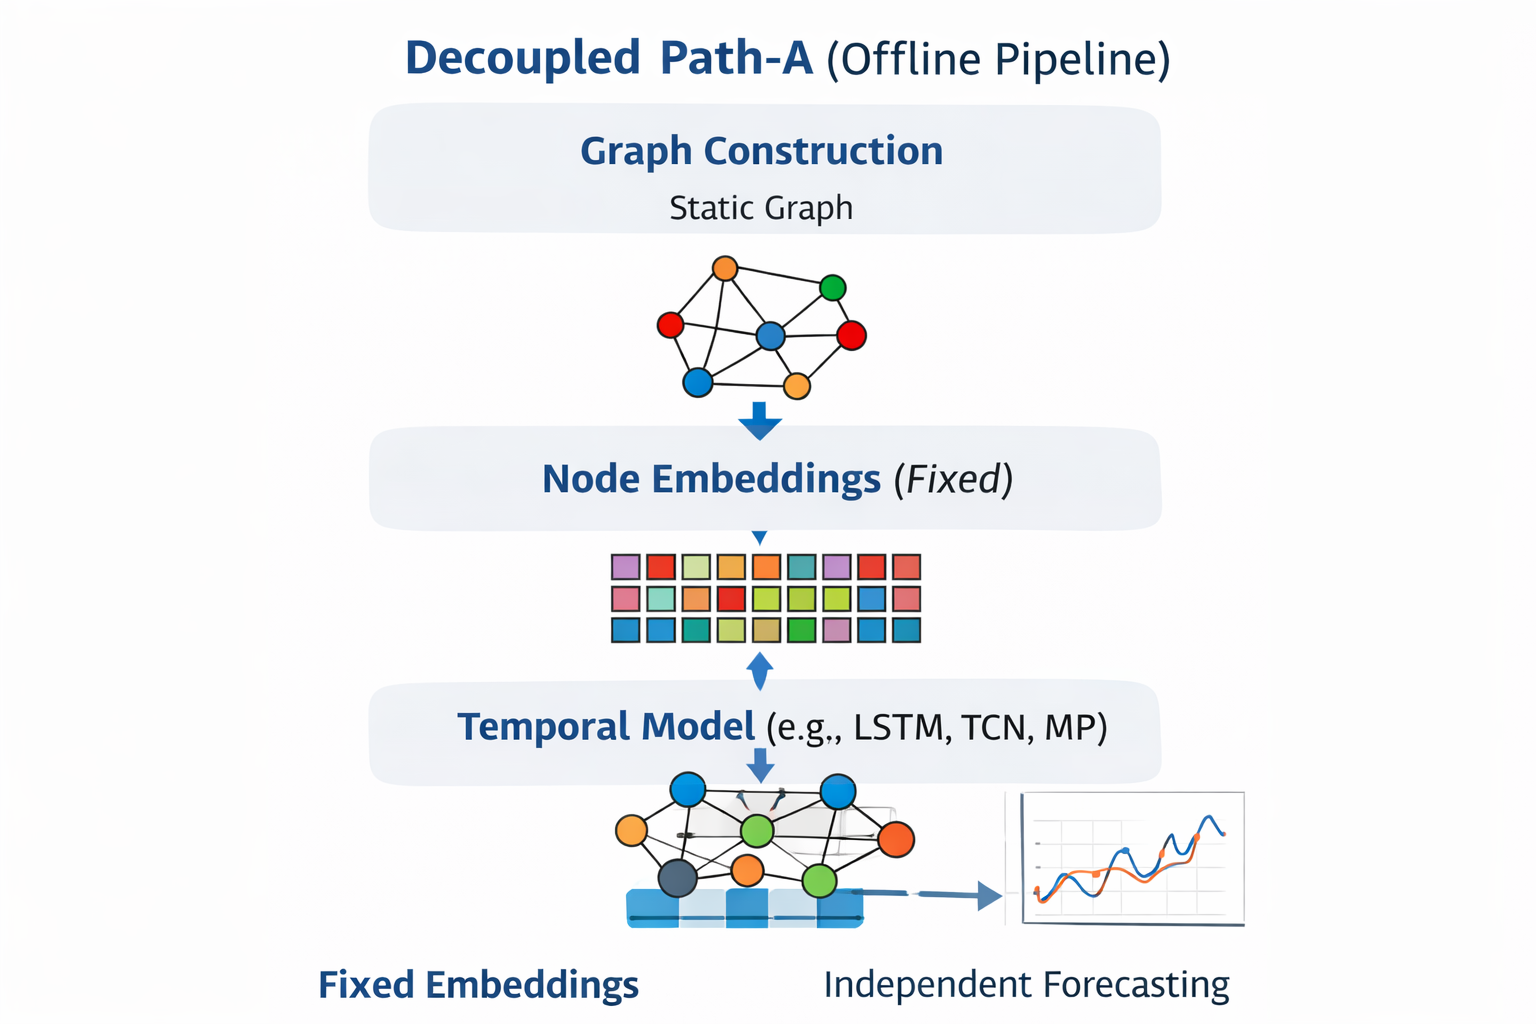
\includegraphics[width=0.5\linewidth]{Decoupled Path-A.png}
    \caption{Decoupled Path_A Architeture}
    \label{fig:pathA-decoupled}
\end{figure}
\fi
\subsection{Integrated Path-A}

In \emph{integrated Path-A} pipelines, the graph is \textbf{constructed} by a \textbf{non-parametric, deterministic, loss-independent} procedure and is \textbf{not updated by the forecasting gradient}. Instead, graphs (and the associated node representations) are \textbf{recomputed over rolling time windows} and supplied as time-indexed relational priors to a forecasting model whose parameters are trained end-to-end on the prediction task.

Specifically, the forecaster may be jointly trained with a graph \emph{encoder} (e.g., a GNN that maps the constructed adjacency to embeddings), but the \emph{construction rule} itself is fixed: it is neither parameterized nor optimized or supervised by the predictive loss. This design improves robustness under nonstationarity by temporally aligning relational information with the forecasting window and is particularly relevant in retail and finance, where dependencies drift over time \cite{wang2022sparsificationfilteringspatialtemporalgnn}. A trade-off is that embeddings become time-dependent, which can reduce cross-time reusability unless additional alignment or stability constraints are imposed on them.

\iffalse
\begin{figure}[h]
    \centering
    \includegraphics[width=0.5\linewidth]{image.png}
    \caption{Decoupled Path_A Architeture}
    \label{fig:pathA-integrated}
\end{figure}
\fi
\subsection{Suitability with Respect to the Research Questions}

Both Path-A variants align with the research questions of this dissertation, addressing them from complementary perspectives.

\paragraph{RQ1: Reusable graph-based representations.}
Decoupled Path-A directly targets reusable task-agnostic node embeddings derived from explicit loss-independent graphs that can be reused across temporal forecasters. Integrated Path-A supports a time-adaptive notion of reuse, in which embeddings remain usable across forecasters while evolving over rolling windows to reflect changing relational dynamics.

\paragraph{RQ2: Integration strategies with temporal models.}
The decoupled vs. integrated distinction provides a principled axis for evaluating how fixed versus time-varying embeddings and offline versus rolling computations affect forecasting accuracy, interpretability, and representation quality.

\paragraph{RQ3: Scalability and robustness in large-scale retail settings.}
Integrated Path-A is particularly relevant because of its ability to accommodate exogenous drivers, seasonality, and catalog changes at the cost of repeated graph/embedding recomputation over time. Decoupled Path-A serves as a strong baseline for computational efficiency under stable relational conditions.

\section{Graph Construction for Retail Demand (Path-A Focus)}
\label{sec:sota-graph-construction}

Retail demand forecasting differs from domains with \emph{physical} relational structure (e.g., road networks in
traffic forecasting) in that product--product dependencies are typically \emph{latent}, \emph{confounded} by shared
drivers (calendar seasonality and promotions), and potentially \emph{time-varying} factors. In the dataset considered in this dissertation, transactional baskets are not observed; therefore, canonical co-purchase graphs are not directly
identifiable. Instead, relational priors must be derived from \textbf{loss-independent} signals available in the data, such as product metadata and hierarchy labels, the similarity of sales trajectories (preferably after controlling for promotion and calendar effects), and shared promotional exposure.

In line with the \textbf{Path-A} paradigm, this section reviews graph construction strategies that are \emph{decoupled}
from downstream forecasting loss. We begin with \textbf{heuristic graphs} that encode simple, interpretable
relations (taxonomy, correlation, promotion co-exposure, and co-activation proxies). We then cover three principled
correlation graph generators that improve stability and sparsity in high-dimensional settings: \textbf{Information Filtering Networks} (topology-constrained filtering), the \textbf{Graphical Lasso} (sparse precision estimation), and
\textbf{covariance shrinkage} (denoising/conditioning). Finally, we discuss \textbf{candidate-edge sparsification} (top-$K$/kNN), which is essential to make dense pairwise scores tractable at retail scale and serves as a common
post-processing step across all the graph constructors.

\subsection{Heuristic Graph Construction Methods}
\label{sec:heuristic_graphs}

Early graph-based approaches to time series modeling rely on heuristic graph construction methods,
in which relational structures are defined using domain knowledge or simple statistics computed
from the data. In these settings, entities such as sensors, regions, or products are represented as
nodes, and edges are established based on predefined similarities or interaction criteria. These methods
are attractive because of their simplicity, interpretability, and low computational costs. In this dissertation, we primarily consider graphs whose nodes correspond to \textbf{SKUs} (one node per \texttt{item\_id}), yielding a global SKU--SKU relational prior that can be reused across stores. When the data are store$\times$item panels, SKU-level dependency scores can be computed from aggregated series (e.g., summed across stores) or by averaging store-level scores.

A common class of heuristic graphs is correlation-based graphs, where edges are constructed using
statistical dependency measures such as Pearson or Spearman correlation coefficients computed between
time series. Such graphs have been widely used in energy consumption forecasting, traffic modeling,
and industrial monitoring, under the assumption that strongly correlated series are likely to exhibit
meaningful interactions. Variants include thresholded correlation graphs, $k$NN correlation graphs,
and lag-aware correlation measures; unless otherwise stated, correlation graphs are treated as weighted
and undirected, with neighborhood selection often based on $|\rho|$, while lag-aware measures may be used
to induce directed edges when peak dependency occurs at a nonzero lag. Some industrial forecasting pipelines
combine a physical graph with an additional behavior-similarity graph constructed from entity time series.
For instance, RCCNet \cite{10.1145/3690649} uses a road network for spatial context but also builds a
courier--courier graph via historical time-series similarity, illustrating a transferable pattern for settings where the relationships are not directly observed.

In retail, an analogous heuristic is an SKU--SKU similarity graph (top-$K$/$k$NN on sales signals, or on
residuals after controlling for calendar and promotion effects), while the route-based physical topology
has no direct counterpart and is not assumed to be present. Practical retail pipelines also rely heavily on $k$NN-style sparsification to control graph density at scale; we return to a representative retail-scale implementation of this principle in Section~\ref{ss:asg-rnn}. Because retail series are often sparse and zero-inflated (due to intermittent demand or temporary unavailability), robust variants may complement correlation on raw counts with similarity computed on the transformed series and/or binary activity indicators.

Another widely adopted heuristic is co-occurrence or co-purchase graph construction, especially prevalent in
retail, and recommendation systems. In such graphs, edges are defined based on the frequency with which products are purchased together, viewed together, or appear within the same transaction basket. These graphs naturally capture complementarity relationships and have been shown to provide useful relational priors for downstream learning tasks. However, in our setting, transaction baskets are not observed (only daily store$\times$item unit sales), so co-purchase graphs are not directly identifiable and must be approximated via co-sale/co-activation proxies (e.g., Jaccard similarity of nonzero-sales indicators within store and time windows), which capture co-occurrence in daily
activity, rather than within-basket complementarity. Category-based graphs represent a related strategy, in which products are connected if they belong to the same category, department, or brand hierarchy, reflecting semantic similarity, as defined by business taxonomies.

In retail environments, promotional and calendar-driven heuristics are also frequently employed. For example,
products may be connected if they are simultaneously affected by the same promotion type, discount mechanism, or seasonal event. These graphs encode business rules and campaign-level dependencies, offering high interpretability and direct alignment with operational expertise.

Heuristic graph construction methods offer several advantages. First, they are scalable to large graphs, as their construction typically involves linear or near-linear complexity concerning the number of entities. Second, they produce interpretable structures that can be inspected and validated by domain experts. Third, they can be constructed independently of downstream forecasting models, thereby enabling modular pipelines.

However, heuristic graphs also exhibit fundamental limitations. In fact, many heuristics are
\emph{instantaneous} and largely \emph{symmetric}: correlation-based graphs can indicate co-movement but do not distinguish direct influence from shared drivers, nor do they naturally encode directionality.
Also, simple similarity measures can be strongly confounded in retail settings by common
seasonality, calendar events, and promotion regimes, yielding dense patterns of spurious edges
unless careful preprocessing and sparsification are applied. 
Product interactions can be \emph{lagged} (effects manifest after several days) and occasionally \emph{nonlinear}, which may not be captured well by linear correlation or taxonomy proximity alone. These limitations motivate augmenting heuristic constructions with richer, yet still loss-independent, dependency estimators that can capture directed and/or nonlinear relations when warranted by the data.

\subsubsection{Information-Theoretic and Causal Dependency Graphs}
Beyond correlation and taxonomy heuristics, loss-independent dependency estimators from time-series analysis and information theory can be used to derive SKU--SKU graphs that capture \emph{directed} and/or \emph{nonlinear} effects.
These methods operate on pairs of series (typically after preprocessing to reduce shared seasonality and promotion confounding) and yield weighted adjacency matrices that can be sparsified via top-$K$/mutual-$K$ selection or filtered backbones. In retail-scale catalogs, candidate-edge restriction (e.g., evaluating expensive estimators only among taxonomy neighbors or top-$K$ correlation candidates) is often necessary to keep computation tractable.

\paragraph{Granger Causality (GC).}
Granger causality induces a \emph{directed} graph by testing whether past values of series $j$ improve the prediction of series $i$ beyond the history of $i$ alone. In its standard form, GC is implemented via autoregressive models (or VAR) and edges are weighted by a test statistic or error-reduction score. GC is attractive in retail because it is explicitly
\emph{lag-aware} and yields directionality, but it can be sensitive to nonstationarity and shared drivers; therefore, GC graphs are preferably computed on detrended/residualized series and within rolling windows.

\paragraph{Mutual Information (MI).}
Mutual information constructs an (often \emph{undirected}) dependency graph by measuring statistical dependence between pairs of series beyond linear correlation. MI can capture nonlinear associations and is thus useful when substitution or co-activation relationships are not well described by correlation. Practical MI estimation in high dimensions typically requires careful discretization or kNN-based estimators and is substantially more expensive than correlation, motivating aggressive sparsification.

\paragraph{Transfer Entropy (TE).}
Transfer entropy measures directed information flow from $j$ to $i$ by quantifying how much the past of $j$ reduces the uncertainty of the future of $i$ beyond the past of $i$. TE yields a \emph{directed, lag-aware} graph and can capture nonlinear effects, but pairwise TE estimation is computationally heavy at retail scale; feasible implementations typically use short rolling windows, low-order embeddings, and/or candidate-edge restriction (e.g., compute TE only among a preselected neighbor set from correlation or taxonomy).

\paragraph{Maximum-likelihood coupling / reconstruction graphs (MLE/MLR).}
Some approaches infer a coupling matrix by fitting a generative or reconstruction model to the multivariate series and interpreting learned cross-series parameters as edge weights. These graphs can capture structured dependencies beyond pairwise similarity, but they introduce additional modeling assumptions and hyperparameters; in Path-A pipelines they are still loss-independent with respect to the downstream forecaster, but their computational cost may require restricting to candidate neighbors or low-rank parameterizations.


While information-theoretic and causal estimators enrich heuristic graphs by introducing directionality, lag structure, and nonlinear dependence, they can be substantially more expensive and sensitive to estimation noise in short windows.
Complementarily, a second class of loss-independent constructors improves \textbf{stability} and \textbf{sparsity} for \emph{correlation/covariance-driven} graphs by applying explicit regularization or topology constraints rather than ad hoc thresholding. The next subsections review three such generators---\textbf{Information Filtering Networks} (IFNs), \textbf{Graphical Lasso}, and \textbf{covariance shrinkage}---which provide stable, interpretable relational priors and serve as practical building blocks for Path-A pipelines at retail scale.

Because retail demand series are strongly affected by shared seasonality, calendar events, and promotional campaigns, these dependency estimators are preferably applied to pre-processed signals whenever possible (e.g., detrended and seasonally adjusted series and/or residuals after controlling for promotion and calendar covariates). This reduces spurious edges induced by global co-movement rather than product-to-product interactions and improves robustness under rolling-window graph refresh.

\subsection{Information Filtering Networks}
\label{subsec:ifn}

Information Filtering Networks (IFNs) are \emph{topology-constrained} graph construction methods that extract sparse and interpretable dependency structures from dense correlation (or covariance) matrices. Their motivation is practical because empirical correlation estimates are typically noisy and fully connected, especially in high-dimensional settings or when only short windows are available. Rather than estimating sparsity via iterative precision-matrix optimization, IFNs \emph{filter} a similarity matrix by retaining only the most informative relations subject to explicit structural constraints, yielding graphs with controlled complexity and strong interpretability \cite{wang2022sparsificationfilteringspatialtemporalgnn}.

IFNs typically start from a similarity matrix, such as a Pearson correlation matrix, and then transform these similarity scores into edge weights that behave like distances. Under this transformation, pairs of nodes with higher similarity (i.e., stronger correlation) are assigned smaller “distances,” whereas weakly related pairs receive larger distances. This distance-like representation is convenient because many IFN constructions (e.g., spanning tree and filtered graph algorithms) naturally select edges by favoring the shortest distances, thereby prioritizing the strongest relationships.


The Minimum Spanning Tree (MST) provides the simplest IFN ``backbone'': it selects $n-1$ edges that connect all nodes while minimizing the total distance, thereby preserving the strongest dependencies under an extreme sparsity constraint. This yields a highly interpretable structure but excludes cycles and, therefore, discards redundant (yet potentially meaningful) relations.


To retain more information while remaining strongly regularized, the IFN variants relax the tree constraint. The Planar Maximally Filtered Graph (PMFG) \cite{tumminello2005pmfg} adds edges in the order of decreasing similarity while enforcing planarity, allowing cycles and clique-like motifs. Chordal IFNs, such as the Triangulated Maximally Filtered Graph (TMFG) \cite{massara2016tmfg}, further enforce decomposable (triangulated) structures, enabling efficient clique-based factorization and supporting sparse, positive-definite precision representations \cite{wang2022sparsificationfilteringspatialtemporalgnn}. 


From a Path-A perspective, IFNs offer a principled way to derive \emph{explicit, deterministic, and loss-independent} relational priors directly from the dense similarity matrices. Their topology-constrained filtering produces \emph{sparse} graphs with controlled complexity, which improves the scalability for large node sets and reduces the sensitivity to noisy correlation estimates. Because the resulting structures are easy to inspect (e.g., backbone edges and clique motifs), IFNs also support interpretability and domain validation, a desirable property in retail settings where analysts may wish to verify whether inferred relations align with known substitution, complementarity, or campaign-level effects. 

In rolling-window regimes, IFNs can be recomputed efficiently to yield \emph{time-local} graphs that track evolving dependency patterns while preserving the modularity. The graph construction stage remains separate from (and unaffected by) the forecasting loss, enabling the reuse of the same graph generator across different temporal models and experimental configurations. Overall, IFNs provide a practical middle ground between naive thresholding (often unstable) and fully learned graph inference (often task-coupled), making them well-suited as Path-A graph constructors in the proposed framework.

It is important to note that IFNs are primarily driven by pairwise similarity and may miss asymmetric or lagged effects unless complemented by directed or lag-aware estimators. In retail, to reduce spurious edges from shared seasonality and campaign-level effects, IFNs are preferably built from pre-processed series (detrending/seasonal adjustment and promotion/calendar controls as noted above). Accordingly, IFN outputs are best interpreted as \emph{filtered dependency priors} rather than as definitive structural models.

\subsection{Graphical Lasso}
\label{subsec:glasso}

The graphical Lasso (GLASSO) is a correlation graph generator that constructs sparse dependency graphs by estimating a sparse \emph{precision} matrix (inverse covariance). Under the Gaussian modeling assumption, nonzero off-diagonal entries of the precision matrix correspond to \emph{conditional} dependencies: an edge between variables $i$ and $j$ indicates that their association remains after accounting for all other variables. This provides a notion of ``direct'' dependency, which is often more informative than raw correlation, which can be inflated by shared global drivers.

Given an empirical covariance matrix $S$, GLASSO estimates a positive definite precision matrix $\Theta \succ 0$ by solving an $\ell_{1}$-regularized maximum likelihood problem \cite{friedman2008glasso}:
\begin{equation}
\hat{\Theta}
=
\arg\min_{\Theta \succ 0}
\Big(
-\log\det(\Theta) + \mathrm{tr}(S\Theta) + \lambda \|\Theta\|_{1}
\Big),
\end{equation}
where $\|\Theta\|_{1}$ denotes the element-wise $\ell_{1}$ norm (typically applied to off-diagonal entries), and $\lambda \ge 0$ controls sparsity. A larger $\lambda$ yields sparser graphs and stronger regularization.


GLASSO produces sparse and interpretable adjacency structures without ad hoc thresholding, a tunable density accuracy trade-off via $\lambda$, and graphs that may be more robust to spurious correlations caused by common factors, as edges reflect conditional rather than marginal associations. When computed over rolling windows, the GLASSO can provide time-local dependency graphs that adapt to nonstationary regimes while remaining loss-independent.


However, GLASSO relies on distributional assumptions (e.g., approximate Gaussianity) and can be sensitive to confounding and non-stationarity. In retail, shared calendar seasonality and promotions can induce widespread co-movement; therefore, it is preferable to estimate $S$ from preprocessed series (detrending/seasonal adjustment and promotion/calendar controls as noted above) to avoid encoding global effects as direct edges. Computationally, the GLASSO involves iterative optimization and may be costly for very large graphs unless sparsity is enforced aggressively or approximate solvers are used.


\subsection{Covariance Shrinkage}
\label{subsec:shrinkage}

Covariance shrinkage is a regularization technique that improves the stability of empirical covariance (or correlation) estimates by shrinking them toward a structured target matrix. The motivation for this is that sample covariance matrices can be poorly conditioned and highly variable when the number of variables is large relative to the available observations (a common situation in high-dimensional retail catalogs or short rolling windows). Shrinkage reduces the estimation variance and yields more reliable similarity weights for graph construction \cite{ledoit2004wellconditioned}.

A standard shrinkage estimator takes the following form:
\begin{equation}
\hat{\Sigma}_{\alpha} = (1-\alpha)\hat{\Sigma} + \alpha T,
\end{equation}
where $\hat{\Sigma}$ is the empirical covariance, $T$ is a target matrix (often a scaled identity), and $\alpha \in [0,1]$ controls the shrinkage intensity of the matrix. By compressing extreme eigenvalues and improving the conditioning, shrinkage produces correlation/covariance matrices that are more numerically stable and less sensitive to sampling noise.

Shrinkage is computationally lightweight and scalable, making it well suited for large graphs and rolling window settings. Although shrinkage does not enforce sparsity, it yields \emph{denoised edge weights} that can be thresholded, kNN-sparsified, or passed to topology-constrained filters, such as IFNs. In Path-A pipelines, shrinkage serves as a robust preprocessing step that improves the quality and stability of correlation-derived graphs and downstream node embeddings.

Shrinkage controls the variance but can introduce bias toward the chosen target, potentially weakening meaningful weak dependencies if $\alpha$ is too large. Because the output is typically dense, additional sparsification is usually required to obtain tractable adjacency matrices for graph encoders. As with other correlation-based methods, retail-specific preprocessing (e.g., seasonal adjustment and promotion control) is recommended to reduce spurious global co-movements.

\subsection{Sparsification and Candidate-Edge Selection (Top-$K$/kNN)}
\label{ss:sparsification-topk}

A practical challenge in retail-scale settings (e.g., $N \approx 10^{4}$ SKUs) is that many graph
constructors yield dense pairwise score matrices (e.g., correlation, covariance, embedding similarity),
which are computationally prohibitive to store and to use downstream (e.g., for neighbor aggregation
or message passing). A widely adopted remedy is \emph{candidate-edge sparsification}, where each node
retains only a bounded number of neighbors according to the ranking criterion. This converts an
$O(N^{2})$ fully connected score matrix into an $O(NK)$ sparse graph, with explicit control over memory
and computation.

A common strategy is \emph{top-$K$ selection by similarity} in an embedding or feature space, optionally
This was followed by normalized neighbor weighting. For example, in knowledge-driven pipelines, entity
embeddings are used to compute cosine similarities, select the top-$K$ most similar neighbors for each
entity and aggregate neighbor features with softmax-normalized weights \cite{9763825}. This pattern
transfers directly to retail when product representations are available (e.g., taxonomy embeddings,
attribute embeddings, or learned temporal embeddings): similarities induce a sparse neighborhood,
and neighbor influence is controlled by a normalized weighting scheme.

A closely related strategy is constructing explicit \emph{$k$NN candidate graphs} and treating $K$ as a
sparsity/quality knob. STEP/TSFormer constructs a $k$NN graph from learned time-series
representations and highlights that $K$ trades off completeness against redundancy: a small $K$ may
miss relevant dependencies, whereas a large $K$ can introduce redundant or noisy edges that degrade
aggregation \cite{10.1145/3534678.3539396}. In large catalogs, this motivates treating top-$K$
sparsification as a first-class module that makes dependency discovery and downstream GNN layers
tractable.

In practice, the ranking criterion can be instantiated in several ways:
\begin{itemize}
    \item top-$K$ by cosine similarity of embeddings;
    \item top-$K$ by a distance metric (e.g., Euclidean distance after standardization);
    \item top-$K$ by absolute dependency score (e.g., $|\rho|$ or a lagged-correlation maximum);
    \item mutual-$k$NN (retain an edge only if both endpoints select each other) to further stabilize neighborhoods.
\end{itemize}
These variants preserve the modular Path-A workflow: the sparsified graph is produced deterministically
from a chosen score function, which is then reused for embedding generation and forecasting.




\section{Graph Embedding Generation}
\label{sec:graph_embedding_generation}

Graph embedding generation focuses on learning low-dimensional vector representations of nodes that preserve the structural, relational, and semantic properties of a graph. Unlike end-to-end forecasting architectures, graph embedding methods aim to produce general-purpose, task-agnostic representations that can be reused in downstream applications. This property makes them particularly relevant for modular forecasting pipelines, where relational representation learning is decoupled from the temporal prediction models.
Unless stated otherwise, we use the term \emph{graph-based embeddings} to denote \emph{node-level embeddings} learned from a graph (one vector per entity) rather than a single graph-level representation.



\subsection{Random-Walk Based Graph Embeddings}

Early graph embedding approaches are based on random walks and distributional learning principles borrowed from the field of natural language processing. Methods such as \emph{DeepWalk} \cite{DBLP:journals/corr/PerozziAS14} and \emph{node2vec} \cite{DBLP:journals/corr/GroverL16} generate node embeddings by simulating random walks on the graph and optimizing a skip-gram objective to preserve the node

DeepWalk treats random walks as sentences and nodes as words, implicitly capturing the community structure and local proximity. node2vec extends this idea by introducing biased random walks that interpolate between breadth-first and depth-first exploration strategies, allowing embeddings to capture both local neighborhoods and global structural roles.

Although these approaches are computationally efficient and easy to implement, they exhibit several limitations. First, they are inherently static and require complete retraining when the graph changes. Second, they operate in a transductive setting, which means that they cannot naturally embed unseen nodes without retraining. Finally, they do not incorporate node attributes or heterogeneous edge types, limiting their expressiveness in complex relational domains, such as retail product networks.

In Path-A pipelines, these embeddings can be learned independently of the forecasting loss and then concatenated to the time-series inputs of a temporal predictor. However, in retail settings with catalog churn and time-varying relations (e.g., promotions), static transductive embeddings may quickly become stale unless recomputed over rolling windows, and they do not naturally support unseen products without requiring retraining.

Despite these limitations, random-walk-based embeddings remain valuable baselines and illustrate the core idea of separating representation learning from downstream prediction tasks.


\subsection{Inductive Graph Neural Network Encoders}

Graph Neural Networks (GNNs) have introduced a paradigm shift by enabling inductive graph representation learning. Models such as \emph{GraphSAGE} learn node embeddings by aggregating features from local neighborhoods using learnable aggregation functions \cite{hamilton2017graphsage}. Unlike random-walk-based methods, GraphSAGE supports inductive generalization, allowing embeddings to be computed for previously unseen nodes based solely on their features and local graph structure.

Similarly, Graph Convolutional Networks (GCN) \cite{kipf2017semi} and Graph Attention Networks (GAT) \cite{velickovic2018graph} can be used as general-purpose graph encoders, learning node representations through message passing without being tied to a specific downstream task. When trained with unsupervised or self-supervised objectives, such as neighborhood reconstruction or contrastive learning \cite{velickovic2019deep, zhu2020deep}, these models produce reusable node embeddings that are suitable for external predictors.

In Path-A pipelines, these encoders can be trained once on the constructed graph (or per rolling window) to produce embeddings that are then used by an external temporal forecaster.

\subsubsection{Pre-trained Time-Series Encoders as Node Feature Generators}
Recent studies have explored self-supervised pretraining to learn \emph{reusable} time-series representations that can be exported as node features for downstream models. A representative example is TSFormer/STEP, which pretrains a transformer encoder with a masked reconstruction objective over \emph{patchified} segments of long historical windows, producing patch-level (and optionally series-level) embeddings that capture long-range periodicity and contextual dynamics \cite{10.1145/3534678.3539396}. These embeddings can be frozen and assigned to each SKU as exogenous representations, enabling   direct integration into independent temporal forecasters (e.g., MLP/LSTM/TCN) as additional features, and/or more stable \emph{candidate} graph construction by building sparse $k$NN neighborhoods in the embedding space rather than relying solely on the raw correlation of sales signals. In retail settings with large catalogs, $k$NN-based candidate graphs also provide a practical scalability mechanism by avoiding dense $N^2$ dependency estimation while retaining data-driven relational priors.

\subsection{Relational Self-Supervised Representations for Multivariate Time Series}
\label{ss:relational-ssl-mts}

Beyond purely temporal pretraining, recent \emph{universal} multivariate time-series (MTS) representation frameworks explicitly inject inter-variable structures into self-supervised objectives. A representative example is COGNet \cite{wang2024cognet}, which combines   a transformer-based masked autoencoder (MAE-style) for long-window reconstruction with (ii) a contrastive learning module that learns representations invariant to data augmentations while remaining discriminative across samples. Crucially, COGNet augments standard time-domain contrastive learning with an additional \emph{graph feature representation block} that aggregates neighboring variable information and is trained with a dedicated \emph{graph contrastive loss}. Conceptually, this design encourages embeddings to encode not only temporal patterns within each variable but also latent cross-variable dependency cues.

From the perspective of this dissertation, such relational self-supervised encoders provide \emph{dependency-sensitive embeddings} that can be exported as reusable node features, which naturally align with Path-A pipelines. Because the representations are learned offline under self-supervised objectives (rather than being optimized jointly with a specific forecasting loss), the resulting embeddings can be consumed by independent downstream forecasters (e.g., LSTM/TCN/MLP) or diagnostic models, enabling a controlled evaluation of representation utility and improved modularity across horizons and forecasting architectures.

COGNet also operationalizes scalability through explicit neighborhood sparsification; instead of aggregating information from all variables, it performs attention-based aggregation over only the \emph{top-$K$} most similar neighbors for each variable (top-$K_1$ in their notation) \cite{wang2024cognet}. This choice is motivated by two practical considerations: in high-dimensional MTS, indiscriminate all-to-all aggregation can inject substantial noise and dilute the influence of truly informative neighbors, and restricting aggregation to top-$K$ bounds the per-node message-passing cost, transforming dense inter-variable scoring into a tractable sparse computation. In Path-A terms, this provides an additional “design pattern” supporting your own candidate-edge module: compute a dependency score (e.g., cosine similarity in an embedding space or correlation-based similarity), retain top-$K$ neighbors per node, and then run a graph encoder on the resulting sparse candidate graph.

\subsection{Dynamic Graph Embedding: Predecessors, Taxonomy, and Design Trade-offs}
\label{subsec:dynamic_embedding_predecessors_deep}

Dynamic graph embedding addresses the problem of learning node representations when the underlying relational structures evolve over time. Compared to static graph embedding, the core difficulty is that the embedding function must balance two competing objectives: \emph{temporal sensitivity}, that is, capturing meaningful changes in node neighborhoods and interaction patterns, and \emph{temporal stability}, that is, maintaining representation continuity so that embeddings remain comparable across time steps. Existing approaches can be broadly organized based on how they represent time and enforce temporal consistency. A useful decomposition is as follows: \emph{(a) temporal graph representation}, \emph{(b) representation learning objective}, and \emph{(c) update mechanism}. Following this view, prior work can be grouped into snapshot-based and sequential-interaction-based approaches, each with distinct implications for modular (Path-A) pipelines.

\subsubsection{Snapshot-Based Dynamic Embedding Approaches}
Snapshot-based methods discretize a dynamic graph into a sequence of static graphs $\{G^{(1)}, \ldots, G^{(T)}\}$, where each snapshot aggregates interactions within a fixed time interval (e.g., days or weeks). This formulation reduces dynamic embedding to repeated static embedding with temporal coupling, but introduces a modeling choice that is rarely innocuous: snapshot granularity controls the bias--variance trade-off between smoothing and responsiveness.

\paragraph{Hierarchical pooling over sequential correlation graphs.}
Beyond the direct evolution of node embeddings, recent MTS representation learning constructs \emph{sequential graphs} to capture the time-varying correlation structure and then applies \emph{hierarchical pooling} to obtain multi-resolution relational summaries. HierCorrPool \cite{wang2024hiercorrpool} builds a sequence of weighted correlation graphs by splitting an MTS sample into feature windows and deriving time-indexed edge weights from feature similarity (followed by normalization), thereby explicitly modeling the correlation drift across windows. It then introduces a correlation pooling module that learns an assignment matrix to coarsen the weighted graphs layer-by-layer, designed to incorporate both node features and edge weights (motivated by the limitations of pooling schemes built for binary graphs). Conceptually, this provides a “local-to-global” relational abstraction aligned with multi-scale dependency modeling; in retail terms, it mirrors the idea of progressively aggregating SKU-level relations into higher-level clusters (e.g., subcategory/category) while allowing effective relation strengths to change over time.
Although originally evaluated for representation learning across MTS tasks, this windowed graph + pooling design can be interpreted as a reusable relational summarizer that can be exported as features in modular (Path-A) pipelines.
Hierarchical correlation pooling provides a principled multi-resolution summary of time-varying dependency graphs; however, in retail-scale catalogs, it typically requires aggressive sparsification (Top-K/kNN candidate edges) and restricted pooling assignments to avoid O(N2) correlation construction and dense pooling overhead.

\paragraph{Incremental snapshot reconstruction and smoothness.}
A prominent family learns embeddings by minimizing the reconstruction losses for each snapshot while constraining the changes across time. DANE \cite{li2017dane} is representative of approaches that jointly embed topology and attributes by reconstructing snapshots and updating embeddings based on structural/attribute drift between consecutive time steps. DynGEM \cite{goyal2018dyngem}  similarly uses deep autoencoders to learn nonlinear embeddings per snapshot while enforcing stability constraints to prevent excessive drift in the embeddings. The TIMERS \cite{zhang2018timers} model uses relative changes in adjacency matrices and incremental SVD to update the embeddings efficiently, explicitly targeting computational feasibility when $|V|$ is large and successive snapshots are similar.

These methods can be interpreted as optimizing a two-term objective:
\[
\mathcal{L} = \underbrace{\sum_{t=1}^{T} \mathcal{L}_{\text{rec}}(G^{(t)}, Z^{(t)})}_{\text{fit each snapshot}}
+ \lambda \underbrace{\sum_{t=2}^{T}\|Z^{(t)}-Z^{(t-1)}\|^2}_{\text{temporal smoothness}},
\]
where $Z^{(t)}$ is the embedding at time $t$. The smoothness term is crucial; without it, embeddings across snapshots may be arbitrarily rotated, harming comparability and reuse.

Another direction explicitly models temporal dependence by learning from a \emph{window} of previous snapshots. Dyngraph2vec \cite{goyal2019dyngraph2vec} uses multiple historical snapshots and deep architectures (autoencoders and recurrent networks) to predict future structures, typically minimizing a loss of the form $\|f(A^{(t-\ell+1)},\ldots,A^{(t)})-A^{(t+1)}\|_F^2$, thereby entangling the embedding learning with a prediction target (often next adjacency). tNodeEmbed \cite{singer2019tnodeembed} learns snapshot-level embeddings using static methods and then fuses them via temporal models, such as LSTMs, to solve downstream tasks (e.g., node classification and link prediction). Attention-based models such as DySAT \cite{sankar2020dysat} and DyHATR \cite{xue2020dyhatr} employ temporal self-attention across snapshot embeddings to capture long-range temporal patterns while still using per-snapshot structural encoders.

EvolveGCN takes a different stance: instead of evolving node embeddings directly, it evolves the \emph{parameters} of a GCN using a recurrent unit (GRU/LSTM). This yields a time-indexed encoder $\theta^{(t)}$ that adapts the message passing behavior across time. Conceptually, this improves expressiveness for nonstationary graphs, but it also makes reuse more nuanced: what is reusable is not a single static embedding, but rather a temporally conditioned embedding function that can be reused.

Snapshot-based methods provide a clear conceptual pathway to Path-A modularity: once embeddings $Z^{(t)}$ are learned, they can be exported and used by any downstream predictor. However, several limitations are associated with forecasting-oriented pipelines. First, snapshotting requires selecting a time scale; in retail, relations can change at multiple rhythms (daily promotions versus seasonal shifts), making a single time scale brittle. Second, many snapshot-based methods are evaluated primarily on link prediction or node classification, and their embedding objectives may not preserve the aspects of the relational structure that are most relevant for downstream forecasting. Third, scalability can be mixed: whereas incremental SVD and stable autoencoder updates are helpful, temporal attention models may become expensive when the number of snapshots is large.
\subsubsection{Generalizing static embeddings via temporal graph models and alternative snapshotting.}
A complementary, loss-independent view is to obtain dynamic node embeddings by composing a graph time-series representation, a simple temporal graph model that encodes cross-snapshot
dependencies, and any static embedding methods.
Jin et al.~\cite{jin2022generalizing} formalize this perspective and systematically evaluate combinations
of the snapshot representations and temporal models. Beyond the standard $\tau$-graph time series
(fixed time-span snapshots), they propose an $\epsilon$-graph time series that fixes the \emph{number of edges}
per snapshot, reducing instability caused by fluctuating event volumes and yielding more robust
performance when the appropriate time scale is unknown.
To inject temporal dependence while remaining task-agnostic, they study lightweight temporal models such as
a \emph{temporal summary graph} (TSG), which aggregates snapshots with recency-weighted edge decay, and a
(weighted) \emph{temporal reachability graph} (WTRG), which collapses temporally valid walks into a weighted
static graph.
From a Path-A standpoint, these mechanisms are attractive because the temporal coupling is explicit and
loss-independent; in this dissertation we primarily adopt the snapshotting insight (robust discretization)
while treating TSG/WTRG-style temporal graph transformations as optional extensions when edge-timestamped
interaction graphs were available.

\subsubsection{Sequential-Interaction-Based Dynamic Embedding Approaches}
Sequential-interaction-based methods avoid discretizing time into snapshots and instead operate directly on streams of timestamped edges $\{(u_i,v_i,t_i)\}$. This formulation is often better aligned with systems in which interactions occur continuously and at irregular intervals.


CTDNE \cite{nguyen2018ctdne} introduced \emph{temporal random walks} that respect time-ordering constraints, producing sequences of nodes analogous to sentences. Embeddings are learned using skip-gram objectives; however, the co-occurrence statistics reflect temporally valid neighborhoods rather than purely topological proximity. node2bits extends the temporal walk concept by incorporating features and using hashing mechanisms to generate compact representations.

Another line models the node dynamics using event intensity functions. HTNE\cite{zuo2018htne} employs Hawkes processes to capture mutual excitation effects (past interactions increase future interaction probability) by linking dynamic embedding to intensity parameters. JODIE \cite{kumar2019jodie} models embed sequential interactions of  users/items in bipartite graphs, predicting how embeddings evolve over time, often focusing on next-interaction prediction rather than global structural preservation.


Interaction-based methods are highly time-sensitive and naturally support irregular temporal patterns, making them attractive for domains with fine-grained events. However, they are frequently optimized for interaction prediction objectives, which can cause representations to encode \emph{who interacts next} rather than \emph{what long-run relational structure exists}. For retail forecasting, where the objective is demand trajectories rather than interaction events, this mismatch can reduce direct usefulness unless the embedding objective is re-designed.


\subsubsection{A Modular View: From Dynamic Embeddings to Path-A Pipelines}
\label{ss:dyn-modular}
A key contribution of the work on generalizing static embeddings to dynamic settings is the articulation of dynamic embedding as a modular composition: choosing a temporal graph representation (e.g., snapshot sequences or edge streams), a temporal consistency mechanism (e.g., smoothing, recurrence, attention, or incremental updates), and a base embedding function (e.g., node2vec/GCN/GraphSAGE). This framing is particularly valuable for Path-A pipelines because it makes explicit that \emph{dynamic representation learning does not require end-to-end forecasting}. Instead, one can learn embeddings under unsupervised/self-supervised (or auxiliary) objectives that enforce stability and structural fidelity, export them, and then attach any temporal forecaster to them.

This modular perspective also clarifies why newer methods, such as DyHINE and DyHANE, are relevant to this dissertation. Compared to earlier snapshot or streaming approaches, they emphasize \emph{inductive embedding} (supporting unseen nodes), \emph{heterogeneity} (multiple node/edge types and semantics), and \emph{efficient updating} (avoiding full retraining). These properties align with retail settings, where product catalogs change, multiple relation types coexist (e.g., category hierarchy, promotion co-exposure, and data-driven dependence graphs), and embeddings must be refreshed frequently without incurring prohibitive costs.

Dynamic Heterogeneous Information Network Embedding (DyHINE) extends inductive embedding learning to dynamic heterogeneous graphs \cite{xie2021dyhine}. It introduces a temporal aggregation mechanism that updates node embeddings based on evolving neighborhood structures, enabling online updates without full retraining and explicitly targeting the maintenance of long-term representation.

DyHANE \cite{martirano2024dyhane} tackles dynamic heterogeneous attributed networks in a graph-continuous learning environment. At each timestamp, it identifies a subset of \emph{influenced nodes} affected by recent topology/attribute changes and combines them with an experience-replay memory buffer from previous steps to update the parameters of a heterogeneous GNN encoder. This replay mechanism mitigates catastrophic forgetting while maintaining up-to-date node representation over time. In the experiments, the encoder was instantiated using a GATv2-based architecture.

Although DyHANE is evaluated on standard downstream tasks in its original setting, its core contribution—maintaining up-to-date node representations under graph evolution without full retraining—is \emph{compatible with} Path-A forecasting pipelines. In this dissertation, the same principle can be operationalized by constructing time-indexed retail graphs from the available signals (e.g., rolling-window co-sale/co-demand proximity, promotion co-exposure, and correlation/partial-correlation graphs computed on promo- and calendar-controlled residuals, optionally filtered via IFNs/GLASSO), periodically refreshing product embeddings using an incremental encoder, and exporting these embeddings as exogenous node features to independent temporal forecasters (LSTM/TCN/MLP/GRU). Empirically, this enables controlled comparisons between static, rolling-window, and incrementally refreshed embeddings, quantifying the trade-off between the update cost, embedding stability, and forecasting gains under catalog churn and nonstationarity.

These dynamic embedding methods are particularly relevant for retail forecasting pipelines, where graphs constructed from co-purchase behavior, shared promotions, and category hierarchies evolve over time. Incremental embedding updates address scalability constraints and enable the robust reuse of graph representations within temporal forecasting models. For \textbf{RQ1}, it clarifies what constitutes \emph{high-quality} reusable embeddings under nonstationarity: representations must remain comparable across time (stability) while tracking meaningful relational changes (sensitivity), and ideally support inductive updates for new nodes (catalog churn). For \textbf{RQ2}, snapshot-based and interaction-based formulations induce distinct integration strategies with temporal forecasters, ranging from frozen embeddings to rolling window embeddings; the snapshot granularity and update frequency become explicit design knobs affecting forecasting accuracy, interpretability, and representation quality. For \textbf{RQ3}, dynamic embedding methods highlight scalability and robustness trade-offs in large retail graphs: incremental updates reduce retraining cost, while windowed recomputation improves adaptation to seasonality, promotions, and regime shifts, with heterogeneous dynamic encoders (e.g., DyHINE/DyHANE) being particularly aligned with frequent catalog changes and multi-relation retail graphs.



\section{Learned-Graph Forecasting Architectures (Path-B, Adjacent)}
\label{sec:learned-graph-pathb}

A major line of research in graph-based forecasting focuses on end-to-end Graph Neural Network (GNN) architectures for
multivariate time series (MTS) forecasting, in which relational dependencies are \emph{learned jointly} with the
forecasting objective. In these models, each variable in an MTS is represented as a node, and the edges encode latent inter-variable dependencies inferred directly from the data. This paradigm emerged to address a key limitation of
earlier deep learning approaches (e.g., LSTNet, TPA-LSTM), which capture temporal dynamics effectively but do not
explicitly models the pairwise relationships between variables. By integrating graph learning and message passing, learned-graph
forecasters provide a relational inductive bias that can improve predictive accuracy when dependencies are latent,
non-spatial, or unknown, a priori.

Although this dissertation is primarily concerned with \textbf{Path-A} (loss-independent graph-first pipelines), Path-B
models are reviewed here as \emph{adjacent} work for two reasons:   they establish strong forecasting baselines in the
learned-graph setting, and they clarify what is gained (and lost) when relational structure is optimized end-to-end,
namely, performance versus modularity and reusability.

\subsection{MTGNN, AGCRN, and GTS}
\label{sec:pathb-mtgnn-agcrn-gts}

Representative learned-graph MTS forecasters include MTGNN~\cite{wu2020connectingdotsmultivariatetime},
AGCRN~\cite{bai2020adaptivegraphconvolutionalrecurrent}, and GTS~\cite{shang2021discretegraphstructurelearning}.
MTGNN introduces a learnable graph structure module that infers a \emph{directed} adjacency matrix via trainable node
embeddings; this learned graph is used by the graph convolution layers to propagate information across variables, whereas temporal convolutions capture sequential patterns. AGCRN builds a node-adaptive mechanism in which each node has a
learnable embedding and the adjacency is dynamically generated from embedding similarity and integrated into a recurrent
forecasting backbone, enabling operations on non-spatial MTS without predefined graphs. GTS advances this direction by
formulating structure learning as latent relational inference inspired by Neural Relational Inference (NRI)~\cite{kipf2018nri},
emphasizing probabilistic graph sampling and discrete relational modeling to improve interpretability of inferred
dependencies. Collectively, these models illustrate the dominant Path-B approach, in which the relational structure is optimized end-to-end with forecasting loss, tightly coupling graph inference, representation learning, and prediction.

\paragraph{Adjacent relevance to Path-A.}
Although MTGNN/AGCRN/GTS are not designed for modular reuse, they highlight two conceptually reusable artifacts:
the learned adjacency (or sampled relational graph), and node representations produced by message passing prior
to the forecasting head. In principle, these artifacts can be exported by freezing the learned graph and/or embeddings
after training and using them as inputs for independent temporal predictors (e.g., LSTM/GRU/TCN/MLP). However, because they are optimized jointly with the forecasting objective, the resulting structures are typically task- and horizon-specific; direct reuse may therefore generalize poorly unless additional constraints (regularization, auxiliary objectives, or stability
mechanisms) are introduced. This motivates the representation-first Path-A focus of this study, where relational priors are constructed independently of the forecasting loss to improve interpretability and reuse across models and horizons.

\subsection{Discrete and Regularized Structure Learning}
\label{sec:pathb-discrete-regularized}

Beyond continuous adjacency learning via embedding similarity, an associated research direction explicitly targets
\emph{sparse} and \emph{discrete} graph discovery to improve interpretability and scalability. Regularized Graph Structure Learning (RGSL)~\cite{Yu20222362} learns an implicit dense similarity matrix from node embeddings and then generates a sparse adjacency by sampling edges with the Gumbel--Softmax trick, enabling end-to-end optimization while retaining an \emph{extractable} discrete graph. RGSL additionally introduces a fusion mechanism that combines an explicit prior graph with the learned implicit graph (e.g., via Laplacian-based mixing), reflecting practical scenarios in which partial domain knowledge and data-driven dependencies should be reconciled. While these methods remain Path-B due to their end-to-end training with the forecasting loss, they provide a useful contrast point for Path-A pipelines: discrete structure learning improves the inspectability of learned relations, yet the resulting graphs may still be tightly coupled to the training regime and task.

\subsection{Retail-Scale Learned-Graph Forecasting: ASG-RNN}
\label{sec:pathb-asg-rnn}

A notable retail-scale learned-graph forecaster is the Attribute-Space Graph Recurrent Network (ASG-RNN)~\cite{MA2024123727}, which proposed a global storeSKU replenishment with quantile outputs. ASG-RNN constructs a sparse SKU--SKU product network via a
\emph{directed $k$NN} graph in a \emph{learned attribute space}: categorical SKU attributes are embedded and distances in that space determine neighbors. The resulting graph is used for gated graph convolution that propagates cross-SKU promotional signals, which are fused into a Seq2Seq recurrent forecaster for multi-horizon quantile prediction.

Conceptually, ASG-RNN is a \emph{hybrid} case. It employs an explicit $k$NN sparsification mechanism (interpretable and scalable), but the similarity metric itself (the learned attribute embedding space) is optimized jointly with the forecasting objective, placing the overall system closer to Path-B than loss-independent heuristic construction. Beyond accuracy, ASG-RNN also provides
practical engineering patterns relevant to retail-scale robustness and efficiency: it constructs a static ``union-of-SKUs'' graph, extracts dynamic store--time subgraphs via masking as assortments evolve, batches multiple store--time episodes through block-diagonal stacking of adjacency matrices, and applies local scaling/normalization and masking so inactive (e.g., all-zero/off-shelf) series do
not dominate training. These design choices serve as implementable references for RQ3 (scalability and robustness), even though the learned representations remain coupled to the forecasting objective.



\section{Extensions and Adjacent Perspectives}
\label{sec:extensions-adjacent}

While the core focus of this dissertation is on \textbf{Path-A} pipelines---loss-independent graph construction and
reusable representation learning for retail demand forecasting---two adjacent research directions provide valuable
context and design inspiration. First, \textbf{causal graph learning} addresses a limitation of correlation-based
graphs by explicitly modeling directionality and information flow, potentially improving robustness under shift.
Second, \textbf{heterogeneous graph modeling} expands the relational vocabulary beyond a single adjacency by
representing multiple entity and relation types (e.g., products, categories, promotions), a natural fit for retail
systems, where dependencies arise from diverse semantic sources. These perspectives are reviewed here as complementary
building blocks, rather than primary methodological pillars.

\subsection{Causal Graph Learning for Multivariate Time Series}
\label{sec:causal-graph-mts}

Beyond correlation- and similarity-driven graph construction, an important line of research focuses on \emph{causal}
graph learning for multivariate time series (MTS) data. The motivation is that statistical correlation alone is often
insufficient to characterize \textbf{directional} and \textbf{asymmetric} dependencies, particularly when influence
propagates with a temporal delay. Causal discovery methods aim to infer directed relationships that better reflect
information flow rather than mere co-movement, yielding relational structures that may be more interpretable and
potentially more robust to distribution shifts.

Early causal approaches for MTS commonly relied on variants of Granger causality, but these methods typically assume
linearity and stationarity, which limits their applicability in nonlinear and nonstationary systems. More recent studies
have adopted information-theoretic measures such as \emph{Transfer Entropy} (TE), which quantifies directed
information transfer without assuming linearity.

CauGNN~\cite{duan2021caugnn} represents an early attempt to integrate TE-based causal discovery into graph-based
forecasting. In CauGNN, TE is used to infer directed relationships and the resulting causal graph is incorporated
into an end-to-end GNN-forecaster. A notable design choice is that bidirectional relations are collapsed by selecting
a dominant direction via subtracting opposite-direction TE values; while this simplifies the graph, it may discard
meaningful reciprocal influences on them.

CGAD (Entropy Causal Graphs for Multivariate Time Series Anomaly Detection)~\cite{febrinanto2025cgad} revisits
TE-based construction and explicitly preserves \textbf{bidirectional} causal information whenever significant flow
exists in both the directions. CGAD treats causal graph generation as a distinct preprocessing stage: TE is computed
between variable pairs to obtain a weighted, directed adjacency encoding causal strength. To address the high cost of
TE estimation on long sequences, CGAD proposes a sampling-based strategy that partitions time series into smaller
segments and averages causal scores across samples, improving scalability relative to the naive all-pairs estimation.

From a modular perspective, TE-based causal graph induction can be interpreted as a \textbf{loss-independent graph
constructor} that is, in principle, compatible with Path-A pipelines: the causal adjacency can be exported and reused
as a relational prior or as an input to a downstream embedding generator. However, causal discovery remains
computationally demanding at scale and sensitive to confounding and nonstationarity---challenges that are particularly
salient in retail, where shared seasonality and promotions can induce widespread, synchronized patterns. Consequently,
causal graphs are treated in this dissertation primarily as an adjacent perspective and a potential extension, rather
than as the core baseline in the main experimental pipeline.

\subsection{Heterogeneous Graph Modeling for Multivariate Time Series}
\label{sec:heterogeneous-graph-mts}

Many real-world relational systems are \emph{heterogeneous}, meaning that entities and/or relations belong to multiple
semantic types. In contrast to homogeneous graphs (single node and edge type), heterogeneous graphs explicitly model
multiple node types, multiple edge types, or both node and edge types. This is especially relevant for domains such as retail, finance,
and knowledge-driven systems, where dependencies arise from diverse sources (e.g., taxonomy membership, substitution,
shared promotions and external knowledge).

In retail-like settings, heterogeneity may arise at multiple levels: nodes can represent different entity types
(products, categories, brands, promotions), and edges can encode qualitatively distinct relations (categorical
membership, co-exposure to campaigns, similarity of demand trajectories, or substitution links). Collapsing such
signals into a single adjacency can lose semantics; heterogeneous graph modeling preserves relation types and enables
type-aware message passing and representation learning.

\subsubsection{Heterogeneous GNN architectures}
Several extensions of GNNs operate explicitly on heterogeneous graphs by introducing relation-specific transformations
or attention mechanisms. For instance, Relational Graph Convolutional Networks (R-GCNs) assign separate parameters to
each relation type, while heterogeneous attention-based models condition attention weights on node and edge types.
Although these architectures have been widely used in knowledge graphs and recommender systems, their adoption in MTS
forecasting remains more limited: many forecasting-oriented GNNs assume homogeneous nodes and rely on a single learned
or predefined adjacency, which may be insufficient when dependencies are multi-source and of different types. Recent retail
applications nonetheless show that typed relational structure can improve predictive performance and highlight a
practical cold-start pattern where tree-based models complement heterogeneous GNNs when history is sparse
\cite{ma2024proactive_return_hgnn}.

\subsubsection{Dynamic and reusable heterogeneous embeddings}
A related line studies heterogeneous \emph{dynamic} embedding, focusing on maintaining up-to-date node representations
as the graph evolves. DyHINE~\cite{xie2021dyhine} extends inductive embedding learning to dynamic heterogeneous
information networks by updating node embeddings via temporal aggregation over changing neighborhoods, emphasizing
long-term embedding maintenance, rather than optimization for a single downstream task. DyHANE~\cite{martirano2024dyhane}
advances this direction in dynamic heterogeneous attributed graphs by combining heterogeneous attention with
incremental updates and experience replay, mitigating catastrophic forgetting while avoiding full retraining as
topology, and attribute drift. Importantly, these embeddings can be learned independently of a forecasting objective, which aligns conceptually with Path-A modular pipelines, even if their direct applicability depends on whether a suitable heterogeneous graph schema and update stream can be defined from the available retail data.

Heterogeneity can also arise from \emph{external} semantic sources beyond observed interactions. Knowledge-Enriched Company Embeddings (KECE)~\cite{ang2021kece}, developed in finance, combine relations from knowledge graphs with text and numerical attributes to learn representations explicitly reused across tasks. This illustrates a transferable
design pattern for retail: product embeddings may be enriched with hierarchical metadata, brand relations, and
promotion descriptors to improve generalization across stores and time horizons.

\subsubsection{Heterogeneous and multi-scale Path-B forecasting}
Some end-to-end forecasting models directly incorporate heterogeneity within Path-B architectures. For instance,
MTHetGNN~\cite{wang2021mthetgnnheterogeneousgraphembedding} models multiple static and dynamic relation types and
combines them with temporal convolution for forecasting; while effective, its learned representations are still
optimized jointly with the forecasting loss, thereby limiting reuse outside the trained system.

Beyond heterogeneity, Path-B research has also explored \emph{multi-scale} dependency learning, motivated by the
observation that inter-series relations can manifest differently across various temporal resolutions. PMEDGN~\cite{Hou2025PMEDGN}
learns multiple time-varying adjacency matrices in parallel at different temporal scales and fuses the resulting graph
convolutions. While such approaches remain task-coupled, the multiscale principle can be translated into Path-A by constructing a family of loss-independent graphs over multiple rolling window lengths and fusing the resulting embeddings before passing them to an independent temporal predictor.

\paragraph{Hypergraph forecasting for group relations.}
Finally, some forecasting models use hypergraphs to represent higher-order interactions that are not naturally captured by pairwise edges. In retail, group drivers, such as campaigns or category events, can simultaneously affect many SKUs, suggesting that higher-order structures may be beneficial when moving beyond pairwise graphs. Probabilistic Hypergraph
Recurrent Neural Networks (PHRNN) model node--hyperedge relations probabilistically and regularize structure learning
with a prior $k$NN hypergraph, enabling uncertainty-aware higher-order dependency modeling. While hypergraph forecasting
is not central to the Path-A pipeline adopted in this dissertation, it provides a principled adjacent perspective on
why promotion-driven relationships may require group-level abstractions.

\section{Evaluation Considerations in Retail}
\label{sec:eval-retail}

Retail demand forecasting is evaluated not only on average predictive accuracy, but also on its
behavior under \emph{operationally critical} regimes and its ability to provide actionable diagnostics.
In particular, retail series are strongly affected by \emph{exogenous interventions} (promotions),
\emph{calendar seasonality}, and \emph{assortment/availability constraints}. As a consequence,
evaluation should explicitly test  robustness under regime shifts and data scarcity, whether
graph-derived representations are actually used by the forecaster (rather than acting as redundant
features), and optionally, whether the uncertainty estimates remain calibrated under nonstationarity.

\subsection{Robustness Regimes: Peak Periods, Cold-Start, and Store Closures}
\label{sec:robustness-regimes}

Retail demand models are typically trained on long spans of \emph{regular} sales patterns; however, the most costly errors occur when supervision is weakest or the distribution shift is strongest. Three recurring regimes are
particularly important: \textbf{peak periods} (e.g., holiday weeks, flash sales), \textbf{cold-start / sparse-history}
items (new or rarely sold SKUs), and \textbf{store closures / structural zeros} (days when demand is deterministically
constrained by availability). These regimes induce \emph{task-level shifts}, wherein the mapping from history and covariates to future demand changes abruptly and may be weakly supported by training data.

\paragraph{Peak periods.}
In \emph{Peak Period Demand Forecasting with Proxy Data: GNN-Enhanced Meta-Learning}~\cite{10495591}, relational
(graph-derived) features provide context for rapid adaptation. For this dissertation, meta-learning itself is best viewed as \emph{adjacent} to the core Path-A pipeline, but it motivates evaluating whether graph-based
representations improve performance specifically in high-demand/peak windows rather than only on average days.

\paragraph{Cold-start / sparse history.}
Cold-start demand forecasting arises when an item has limited or no historical sales data, making purely temporal signals insufficient. A common response is to transfer information through a \emph{shared structure} such as product taxonomies, shared promotional exposure, or dependence graphs derived from historical co-movements. In the Path-A
framing, cold-start is a primary justification for \emph{decoupled} pipelines: embeddings learned from global relational structure can be computed for all SKUs (including newly introduced SKUs, given attributes and neighborhood
links) and exported as exogenous features for independent temporal forecasters. A related pattern is relation-aware
meta-learning (e.g., RMLDP~\cite{rmldp}), where relations bias transferable initialization toward similar targets. In our setting, basket co-occurrence is not observed, but the same principle can be approximated using taxonomy links, promotion co-exposure, or the similarity of de-seasonalized sales trajectories.

\paragraph{Store closures / structural zeros.}
Closures create a regime where the target is not merely low but \emph{deterministically constrained}. Treating closure days as ordinary observations can yield false-positive sales forecasts on closed days and excessive shrinkage toward zero, which harms accuracy around reopening transitions. Robust pipelines often separate
\emph{availability} from \emph{intensity} using a two-stage (hurdle) decomposition:
\begin{enumerate}
    \item \textbf{Availability model:} predict whether a store--item is open/active using calendar and store-state covariates.
    \item \textbf{Demand-given-open model:} forecast demand conditional on being open, using temporal history and relational features.
\end{enumerate}
Alternatively, closures may be handled via a hard business rule (clamping predictions to zero under a closure flag) while training the demand model, mainly on open days. This remains compatible with Path-A modularity: availability indicators are treated as exogenous covariates, whereas graph construction and embedding generation remain unchanged.

\paragraph{Reusable design patterns for this dissertation.}
Even without adopting full meta-learning pipelines, several patterns from the robustness literature transfer directly:
\begin{itemize}
  \item \textbf{Proxy-task sampling}: train on non-peak windows, test on peak windows.
  \item \textbf{Relational conditioning}: gated fusion or feature-wise modulation rather than only concatenation.
  \item \textbf{Locality for scalability}: $K$-hop ego-subgraphs or top-$K$ neighborhoods.
  \item \textbf{Structural-zero handling}: explicit availability signals or two-stage modeling.
\end{itemize}

A concrete retail-scale engineering reference is ASG-RNN~\cite{MA2024123727}, which constructs a static union-of-SKUs
product graph, extracts store--time subgraphs via masking to reflect changing assortments, batches multiple store--time
episodes via block-diagonal adjacency stacking, and applies masking/normalization so inactive series do not dominate
training. These mechanisms provide implementable guidance for robustness at scale, even though ASG-RNN is a Path-B
learned-graph forecaster.

\subsection{Explainability and Diagnostic Analysis}
\label{ss:explainability}

Beyond improving accuracy, retail demand forecasting models should provide diagnostics that help practitioners understand \emph{why} predictions change under promotions, calendar effects, and regime shifts (e.g., holiday peaks, or store closures). This is particularly important in Path-A pipelines, where graph construction and representation learning are modular and reusable. Therefore, explainability should validate that the temporal forecaster actually \emph{uses} the exported graph-derived embeddings and exogenous covariates and  reveals whether performance gains arise from meaningful promotional or relational signals rather than spurious correlations.

A practical post-hoc approach is \emph{feature attribution} for temporal forecasters. Integrated Gradients (IG) \cite{sundararajan2017axiomatic} is a widely used gradient-based attribution method that quantifies the contribution of each input feature to a model’s prediction by integrating the gradients along a path from a baseline input to the observed input. In this dissertation, IG can be applied to forecasting models that consume (a) lagged sales features, (b) promotion and calendar covariates, and (c) graph-derived embeddings (e.g., Node2Vec or GNN encoder outputs). Aggregating IG attributions over time and across SKUs enables both global and local analyses: globally, one can report which feature groups dominate predictions (e.g., promotion indicators vs. relational embeddings); locally, one can explain individual forecasts during peak periods or sparse-history settings by identifying the most influential promotion types, calendar events or embedding dimensions.

Importantly, IG complements (rather than replaces) the model ablations. While ablations quantify the \emph{predictive utility} of adding embeddings or particular graphs, IG provides a diagnostic view of \emph{how} the forecaster allocates reliance across the feature families. This supports \textbf{RQ2} by comparing integration strategies (e.g., concatenation vs. gated fusion) through attribution mass on embeddings and supports \textbf{RQ3} by examining whether reliance shifts toward relational representations under cold-start, peak events, or nonstationary regimes. Because the IG is post hoc and does not alter the graph construction procedure, it remains compatible with modular Path-A pipelines and can be reported as an interpretability layer on top of the forecasting models.

A related retail-oriented example is a coffee consumption forecasting study, which employs Integrated Gradients as a post-hoc attribution tool to rank input variables by their contribution to the model’s predictions. Based on the resulting attribution scores, the authors selected a consistent top-$k$ subset of influential features and used this reduced feature\cite{11268605} set to stabilize model training and facilitate interpretation across alternative GNN architectures. This illustrates a practical workflow that is directly transferable to store$\times$item demand forecasting: IG can be used not only for explanation, but also as a diagnostic feature-hygiene step to identify redundant covariates and to compare the relative influence of promotion indicators, calendar variables, and graph-derived embeddings, across models. 
\subsection{Uncertainty Quantification via Relational Conformal Prediction}
\label{ss:relational-conformal}

Point forecasts alone are often insufficient for retail decision-making, where planners must trade off stockout risk against overstocking under promotions, calendar effects, and regime shifts. In addition to explaining \emph{why} a forecast changes, it is therefore useful to quantify \emph{how uncertain} the forecast is, ideally with statistical guarantees that remain valid under weak distributional assumptions.

Conformal prediction provides a distribution-free framework for constructing prediction intervals with finite-sample coverage guarantees by calibrating \emph{conformity scores} (typically based on forecast residuals) on a held-out calibration set \cite{vovk2005algorithmic,romano2019conformalized}. However, standard conformal approaches for time series often treat each target series independently, ignoring cross-series dependence when calibrating the uncertainty. This can be suboptimal in multivariate settings, where prediction errors are correlated across related entities (e.g., products affected by the same promotion type or seasonal event).

Relational conformal prediction addresses this limitation by incorporating a relational inductive bias, implemented via graph deep learning operators, directly into the calibration procedure. In particular, Conformal Relational Prediction (COREL) constructs prediction intervals by leveraging information from correlated time series through learned or constructed graph structures, does not require the graph to be known a priori, and can be applied as a post-hoc uncertainty layer on top of any pre-trained predictor \cite{cini2025relationalconformalpredictioncorrelated}. Practically, this means that a retail forecaster (e.g., LSTM/TCN/MLP/GRU consuming sales history, covariates, and graph-derived embeddings) can be trained for point prediction first, after which conformal calibration is performed using residuals while allowing related products to share uncertainty information via graph operators.

For this dissertation, relational conformal prediction is best viewed as a \emph{Path-A-compatible add-on}: it preserves modularity (it does not change the graph construction or embedding generation pipeline) while extending the evaluation beyond accuracy to include calibration metrics such as empirical coverage and interval width. Moreover, adaptive variants can be used with rolling calibration windows to better handle non-exchangeable data and distribution shifts (e.g., during peak periods), aligning uncertainty estimation with real retail nonstationarity \cite{gibbs2021adaptiveconformalinferencedistribution}.

